\documentclass[tikz,border=3pt]{standalone}
\usepackage{amsmath,amssymb}
\usetikzlibrary{arrows.meta,calc}
\definecolor{curveblue}{HTML}{245C86}
\definecolor{accent}{HTML}{A65E2E}
\definecolor{curveteal}{HTML}{287B6D}
\definecolor{curveviolet}{HTML}{76578B}
\begin{document}
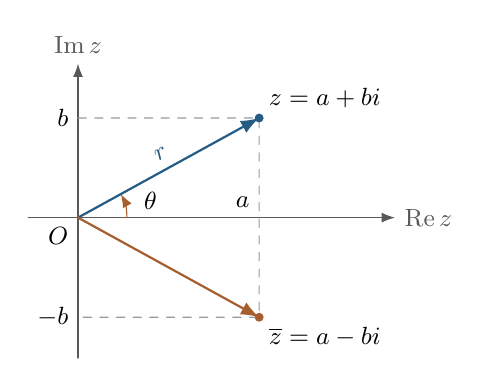
\begin{tikzpicture}[font=\small,>=Latex,line cap=round,line join=round]

\begin{scope}[scale=1.15]
\draw[->,black!65] (-.55,0)--(3.5,0) node[right]{$\operatorname{Re}z$};
\draw[->,black!65] (0,-1.55)--(0,1.7) node[above]{$\operatorname{Im}z$};
\coordinate (Z) at (2,1.1);\coordinate (Zbar) at (2,-1.1);
\draw[black!40,dashed] (0,1.1)--(Z)--(Zbar)--(0,-1.1);
\draw[->,curveblue,thick] (0,0)--node[above,sloped]{$r$}(Z);
\draw[->,accent,thick] (0,0)--(Zbar);
\draw[accent,->] (.54,0) arc[start angle=0,end angle=28.8108,radius=.54];
\node at (.8,.18) {$\theta$};
\fill[curveblue] (Z) circle (1.4pt);\fill[accent] (Zbar) circle (1.4pt);
\node[above right] at (Z) {$z=a+bi$};
\node[below right] at (Zbar) {$\overline z=a-bi$};
\node[below left] at (0,0) {$O$};\node[above left] at (2,0) {$a$};
\node[left] at (0,1.1) {$b$};\node[left] at (0,-1.1) {$-b$};
\end{scope}
\end{tikzpicture}
\end{document}
